\documentclass[tikz,border=9pt]{standalone}
\usepackage{amsmath}
\usetikzlibrary{arrows.meta,calc}
\definecolor{ink}{HTML}{21352F}
\definecolor{teal}{HTML}{087F7B}
\definecolor{blue}{HTML}{4B77A8}
\definecolor{gold}{HTML}{C58B2A}
\definecolor{rose}{HTML}{B65A62}
\begin{document}
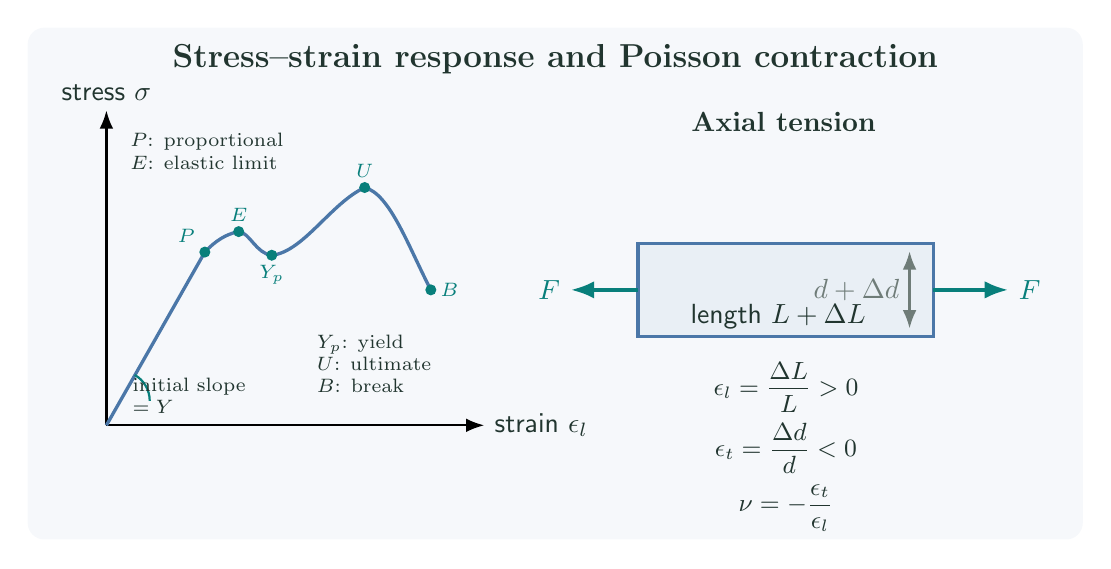
\begin{tikzpicture}[font=\sffamily,text=ink,>=Latex]
  \fill[blue!5,rounded corners=6pt] (-6.7,-3.30) rectangle (6.7,3.2);
  \node[font=\bfseries\large] at (0,2.8)
    {Stress--strain response and Poisson contraction};

  \begin{scope}[shift={(-5.7,-1.85)}]
    \draw[->,thick] (0,0)--(4.8,0) node[right] {strain $\epsilon_l$};
    \draw[->,thick] (0,0)--(0,4.0) node[above] {stress $\sigma$};
    \draw[blue,very thick]
      (0,0)--(1.25,2.2)
      .. controls (1.38,2.34) and (1.52,2.43) .. (1.68,2.46)
      .. controls (1.82,2.45) and (1.90,2.18) .. (2.10,2.16)
      .. controls (2.50,2.20) and (2.85,2.82) .. (3.28,3.02)
      .. controls (3.60,2.94) and (3.83,2.28) .. (4.12,1.72);

    \foreach \name/\x/\y/\place in {
      P/1.25/2.20/above left,
      E/1.68/2.46/above,
      Y_p/2.10/2.16/below,
      U/3.28/3.02/above,
      B/4.12/1.72/right}
      {\fill[teal] (\x,\y) circle (2pt)
       node[\place,font=\scriptsize] {$\name$};}

    \draw[teal,thick] (.36,.64) arc[start angle=60,end angle=0,radius=.38];
    \node[font=\scriptsize,align=left] at (1.05,.38)
      {initial slope\\$=Y$};
    \node[font=\scriptsize,align=left,anchor=west] at (.18,3.48)
      {$P$: proportional\\$E$: elastic limit};
    \node[font=\scriptsize,align=left,anchor=west] at (2.55,.78)
      {$Y_p$: yield\\$U$: ultimate\\$B$: break};
  \end{scope}

  \begin{scope}[shift={(1.05,-.72)}]
    \node[font=\bfseries] at (1.85,2.72) {Axial tension};
    \draw[fill=blue!12,draw=blue,very thick] (0,0) rectangle (3.75,1.18);
    \draw[->,teal,very thick] (0,.59)--(-.85,.59) node[left] {$F$};
    \draw[->,teal,very thick] (3.75,.59)--(4.70,.59) node[right] {$F$};
    \node at (1.78,.25) {length $L+\Delta L$};
    \draw[<->,ink!65,thick] (3.45,.10)--(3.45,1.08)
      node[midway,left] {$d+\Delta d$};

    \node[align=center,font=\small] at (1.88,-1.40)
      {$\displaystyle \epsilon_l=\frac{\Delta L}{L}>0$\\[3pt]
       $\displaystyle \epsilon_t=\frac{\Delta d}{d}<0$\\[3pt]
       $\displaystyle \nu=-\frac{\epsilon_t}{\epsilon_l}$};
  \end{scope}
\end{tikzpicture}
\end{document}
